% unit7.tex
\chapter{开源鸿蒙数据采集与智能控制开发}
\section{传感器数据采集与处理}
\subsection{开发平台介绍}
开源鸿蒙（OpenHarmony）在系统架构中提供了完善的传感器服务框架，使北向应用开发者能够以统一的接口方式访问不同类型的硬件传感器。图\ref{fig:unit7_board_show}所示为开源鸿蒙官方认证的明星开发板——PurplePi OH鸿蒙开发板。该开发板集成了丰富的硬件接口和传感器模块，为北向应用开发提供了良好的实验平台。板载多种接口包括 GPIO、PWM、I²C、SPI 以及串口（USART）通信等，能够满足传感器采集、智能控制以及多设备联动等多样化开发需求。同时，PurplePi OH 支持预装当前最新的OpenHarmony-6.1系统，提供标准化的系统服务和北向 API，使开发者可以快速实现传感器数据采集、执行器控制和多媒体交互功能，而无需关心底层驱动差异。此外，开发板在体积、功耗和扩展性方面均表现优秀，适合在教育、科研及物联网应用开发中进行快速实验和验证。

\begin{figure}[H]
  \centering
  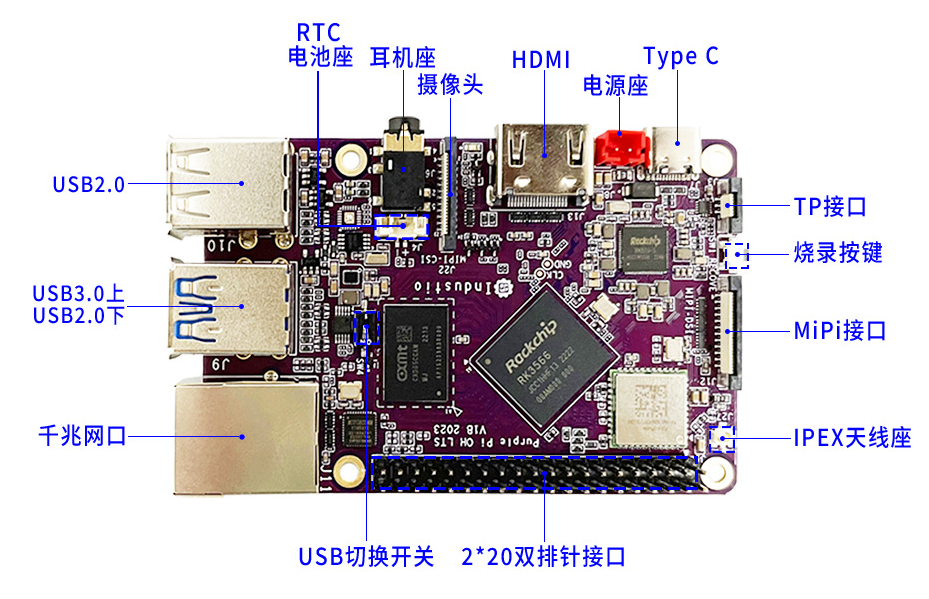
\includegraphics[width=1\textwidth]{images/unit7/board.png}
  \caption{PurplePi OH鸿蒙开发板}
  \label{fig:unit7_board_show}
\end{figure}

此外，根据图\ref{fig:unit7_board_show}开发板设计的开源鸿蒙实训箱，如图\ref{fig:unit7_box_show}所示。学习者可结合后续章节的实践任务，通过北向标准系统扩展板完成对加速度、陀螺仪、光照等典型传感器的数据采集与处理进行讲解，使学习者逐步掌握环境数据读取、信号预处理以及与应用逻辑结合的完整过程。学习者能通过设计APP人机交互操纵执行数据的采集的与处理。

\begin{figure}
  \centering
  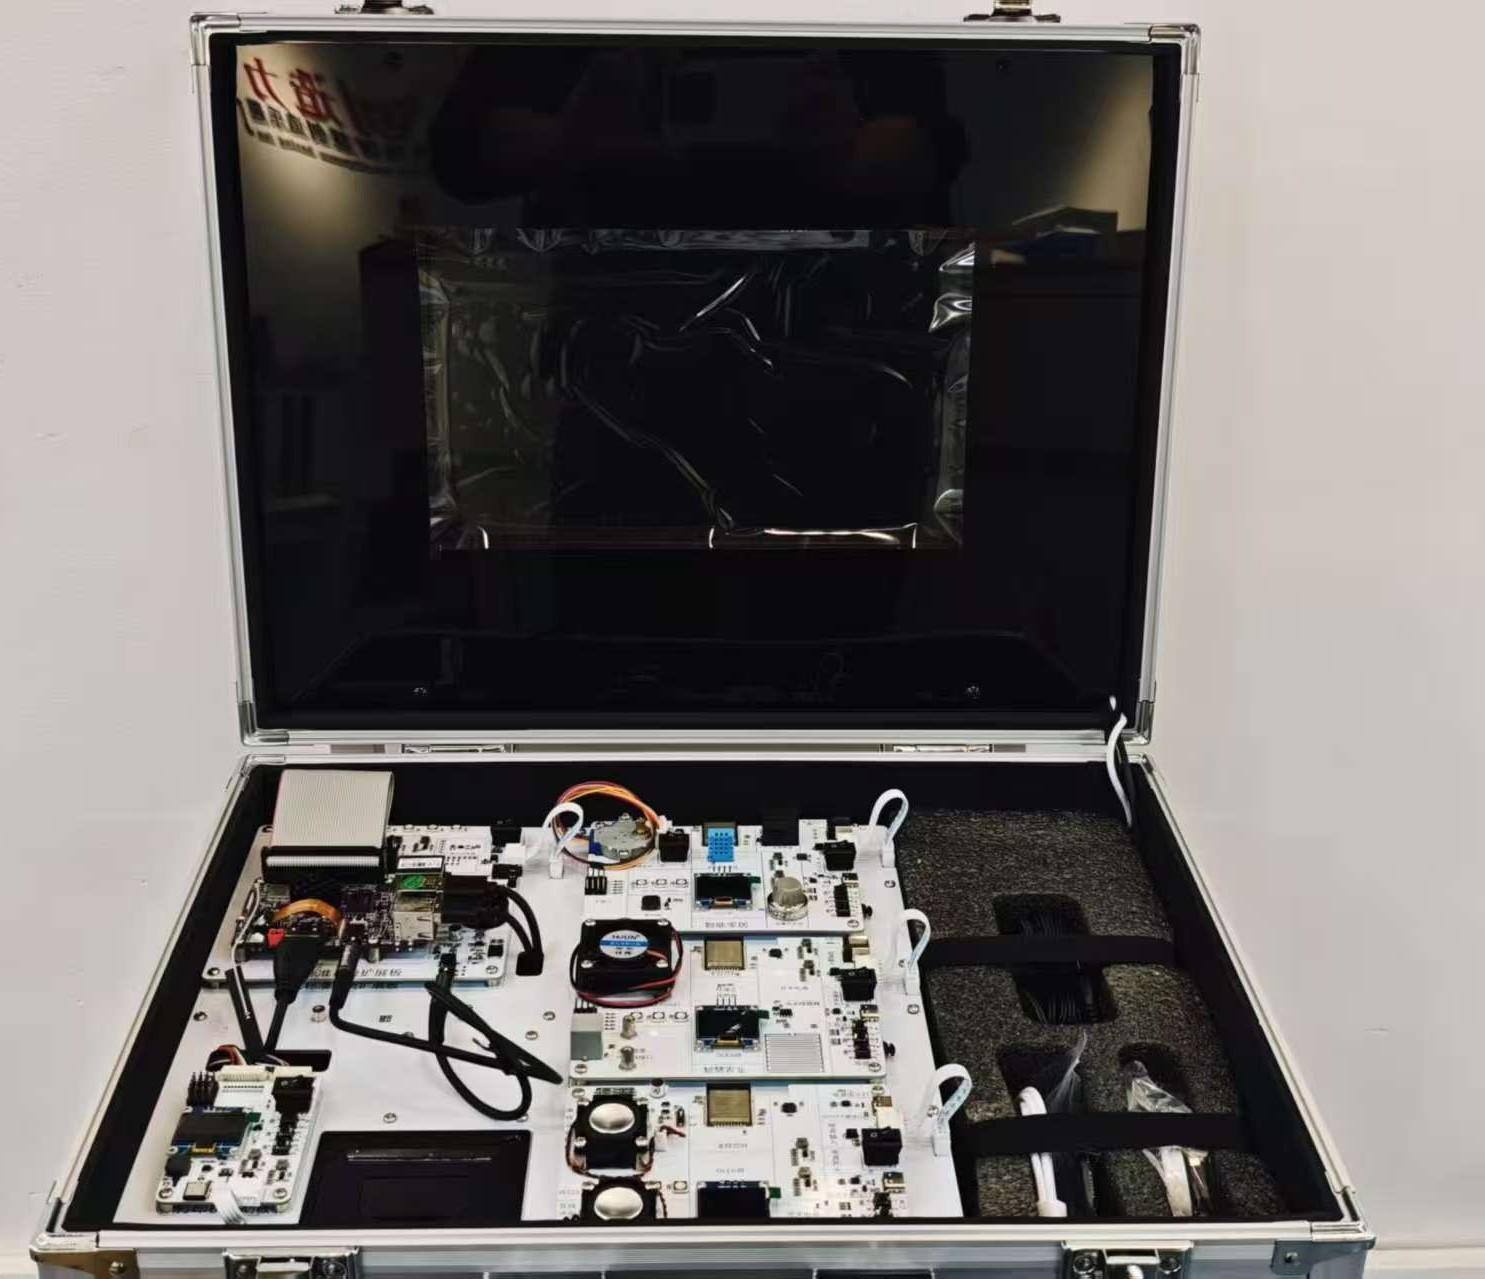
\includegraphics[width=0.8\textwidth]{images/unit7/box.jpg}
  \caption{开源鸿蒙实训箱}
  \label{fig:unit7_box_show}
\end{figure}

\subsection{传感器数据采集}
在智能设备与物联网系统中，环境感知是系统实现自主判断和智能控制的基础能力。在 OpenHarmony 中，传感器的调用基于系统层封装的统一接口。应用程序只需通过北向 API 引入传感器模块，即可向系统注册监听，实现对数据的实时订阅。如图\ref{fig:unit7_sensor_framework}以加速度计为例，应用通过订阅方式获取设备在三轴方向上的加速度变化，系统在传感器更新时主动推送数据给应用层。

\begin{figure}[H]
  \centering
  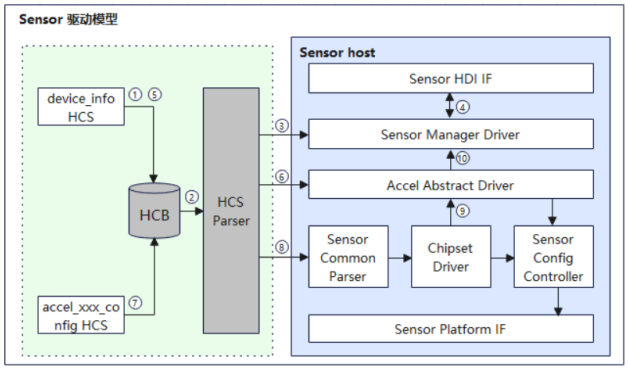
\includegraphics[width=0.85\textwidth]{images/unit7/framework.png}
  \caption{Sensor驱动模型}
  \label{fig:unit7_sensor_framework}
\end{figure}

开发者只需在代码中编写回调函数处理这些数值，即能实现设备姿态检测、动作分析或环境变化监测等功能。例如，应用引入传感器模块后，通过订阅接口即可持续接收加速度的 x、y、z 三轴数据；当不再需要数据时，只需调用取消订阅函数即可释放资源。整个过程采用事件监听模式，数据流的管理由系统完成，开发者仅需关注自身业务逻辑的实现。

以加速度传感器驱动为例，Sensor驱动模型的加载以及运行流程如下：
\begin{myenum}
    \item 从device info HCS 的Sensor Host读取Sensor设备管理配置信息。
    \item HDF配置框架从HCB数据库解析Sensor设备管理配置信息，并关联对应设备驱动。
    \item 加载并初始化Sensor设备管理驱动。
    \item Sensor设备管理驱动向HDI发布Sensor基础能力接口。
    \item 从device info HCS 的Sensor Host读取加速度传感器驱动配置信息。
    \item 加载加速度传感器抽象驱动，调用初始化接口，完成Sensor器件驱动资源分配和数据处理队列创建。
    \item 从accel_xxx_config HCS读取加速度传感器差异化驱动配置和私有化配置信息。
    \item 加速度传感器差异化驱动，调用通用配置解析接口，完成器件属性信息解析，器件寄存器解析。
    \item 加速度传感器差异化驱动完成器件探测，并分配加速度传感器配置资源，完成加速度传感器差异化接口注册。
    \item 加速度传感器探测成功之后，加速度传感器差异化驱动通知加速度传感器抽象驱动，注册加速度传感器设备到Sensor设备管理中。
\end{myenum} 

Sensor驱动模型包括三种驱动：Sensor设备管理驱动、传感器抽象驱动、传感器差异化驱动。

OpenHarmony自带有Sensor设备管理驱动，所以基于Sensor驱动模型开发某一类传感器驱动，需要实现对应的传感器抽象驱动、传感器差异化驱动，以环境光传感器为例，需要实现：环境光传感器抽象驱动、环境光传感器差异化驱动。

\begin{lstlisting}
// 打印信息，用于打印普通信息
#define PRINT_INFO(fmt, args...)    printf("%s, %d, info: "fmt, __func__, __LINE__, ##args)
// 打印信息，用于打印错误信息
#define PRINT_ERROR(fmt, args...)   printf("%s, %d, error: "fmt, __func__, __LINE__, ##args)
\end{lstlisting}
\subsection{传感器数据处理方法}
由于传感器数据常带有抖动和噪声，因此在数据进入应用逻辑之前，需要进行适当的预处理。常见的处理方式包括滑动平均滤波、限幅修正以及基于阈值的事件判断。滑动平均法通过保留若干连续样本计算平均值，能够有效平滑短时间内的波动，使曲线更稳定；限幅方法则用于过滤超出合理范围的错误值，特别适用于光照或温度类传感器的瞬时跳变情况；阈值判断机制常用于实现事件触发，例如在运动检测中，当任一方向的加速度变化超过设定阈值时，即可判断设备发生剧烈摇动，从而触发对应反馈。通过这些处理手段，开发者可以在数据真实性与系统灵敏度之间取得良好平衡。

在智能终端和物联网应用中，传感器采集的原始数据通常包含噪声、抖动或偶发异常值，因此在进入应用逻辑之前需要进行适当的处理，以保证数据的稳定性和可靠性。数据处理的目标在于平滑波动、去除异常、并提取能够反映真实环境状态的有用信息，从而为姿态判断、动作识别或环境监测提供准确依据。

一种常用的方法是滑动平均滤波。滑动平均滤波通过对连续若干个数据样本取平均值来平滑瞬时波动，从而减少短期噪声的影响。该方法实现简单且计算开销小，适用于对变化不特别快速的传感器数据，如加速度计的轻微震动或光照传感器的缓慢变化。滑动平均可以在保证响应速度的同时，提高数据曲线的稳定性，使后续逻辑判断更可靠。

限幅处理是另一种常用的数据处理手段，用于去除明显超出合理范围的异常值。这种方法通过设定上下限，将超过范围的数据裁剪到允许的边界内，避免偶发错误影响系统决策。例如，温湿度传感器在瞬时干扰或硬件抖动情况下可能产生异常读数，限幅处理可以有效消除这种影响，从而保证数据的连续性和安全性。

除了平滑和限幅外，阈值判断在事件检测中也起到重要作用。通过设置合理的阈值，系统可以识别特定事件的发生，例如设备的剧烈摇动、光照不足或温度超标。当传感器数据超过预设阈值时，应用即可触发对应逻辑，实现对环境或设备状态的实时响应。阈值判断方法既直观又高效，尤其适用于运动检测或报警提示等场景。

在实际开发中，这些方法通常可以组合使用，以获得更稳定且可靠的传感器数据流。例如，先对数据进行滑动平均平滑，再进行限幅处理，最后通过阈值判断触发事件。这样的处理流程既能减少噪声对系统判断的干扰，又能够保证事件响应的及时性和准确性。通过合理的数据处理，开发者可以在保证系统灵敏度的同时，提高传感器数据的可信度，为智能应用提供坚实的数据基础。
\subsection{传感器数据传输}
在直接连接的情况下，数据传输过程非常简单。当连接建立成功后，节点 B 会将需要传输的数据封装成符合相应协议格式的数据包，并通过 WiFi 网络发送给节点 C。节点 C 接收到这些数据包后，进行解包和处理，从而完成数据的传递与应用端的使用。

在跨协议设备间的数据传输过程中，流程则更为复杂。首先，节点 D 将需要传输的数据封装成符合 WiFi 协议格式的数据包，并通过 WiFi 网络发送给主节点 A。主节点 A 接收到来自 D 的数据包后，解析其中内容，并根据目标节点 C 的 IP 地址或其他标识信息，将数据重新封装成适合在网络中传输的格式，再通过 WiFi 网络发送给 C。随后，节点 C 接收到 A 转发的数据后，将其从 WiFi 协议格式转换为蓝牙协议格式，并通过事先建立的蓝牙连接将数据包发送给最终目标节点 E。整个过程实现了不同通信协议和设备间的无缝数据传输，保证了信息在多节点、多协议网络中的正确传递与处理。

为了更具体地展示传感器数据采集与处理的流程，本任务以“加速度计的摇动检测”为实例，给出完整的开发过程。应用首先创建缓冲区记录数值变化，通过滑动平均法对加速度数据进行平滑处理，然后将处理后的数据代入判断逻辑。当任一方向的加速度绝对值超过经验阈值时，即可认为发生摇动动作，并在应用界面或日志输出中进行提示。该示例不仅展示了北向 API 的使用方法，也体现了传感器数据预处理的重要性，为读者后续实现更复杂的动作识别或环境感知功能提供基础。
\section{电子罗盘数据采集}
\subsection{电子罗盘数据功能简介}
电子罗盘作为移动设备中常用的方向感知传感器，通过测量地磁场的三轴分量，帮助系统判断设备当前所处的方位角。在许多智能终端场景中，例如导航定位、地图旋转、方向指示、增强现实渲染以及农业巡检路径规划等功能，都依赖电子罗盘提供稳定、实时的方位信息。OpenHarmony 在传感器框架中同样对电子罗盘进行了抽象封装，使北向应用开发者能够通过统一接口获取磁场数据，并构建相应的方向感知功能。本任务将围绕罗盘数据的采集、校准和应用场景展开，帮助读者理解其工作机理并掌握开发方法。

\begin{figure}[H]
  \centering
  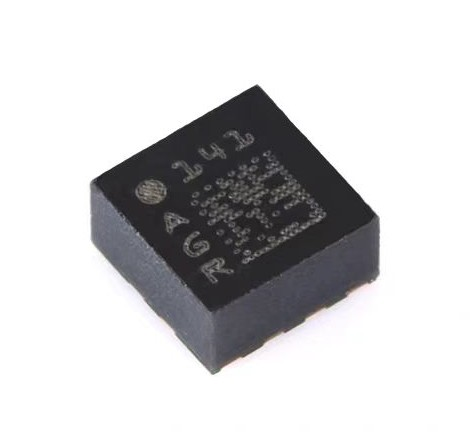
\includegraphics[width=0.6\textwidth]{images/unit7/compass.jpg}
  \caption{电子罗盘实物图}
  \label{fig:unit7_compass}
\end{figure}

在数据采集层面，电子罗盘与加速度计一样，采用事件订阅的方式提供实时数据。应用首先向系统注册罗盘传感器监听，系统随后会按照用户设定的采样频率推送最新的地磁矢量值。收到数据后，应用可从中获取磁场在 x、y、z 三个方向上的分量，通过数学运算转换为设备的方向角。例如，利用反正切函数可以计算水平方向的偏航角，用以表示设备朝向。整个过程依赖稳定的数据来源，而 OpenHarmony 的传感器服务为应用提供了持续且高可靠性的地磁数据通道，极大简化了方向感知功能的实现。

然而，由于受周围环境的磁干扰影响，电子罗盘的数据往往会出现漂移、偏移甚至局部失真。常见干扰来源包括金属外壳、强磁性物体、电机设备、线路电流变化等。因此，在罗盘数据进入应用逻辑之前，通常需要进行校准和补偿。校准方法包括自动校准和用户引导校准。自动校准由系统通过监测磁场变化自动完成，而用户引导校准则常通过手势提示，要求用户以“∞”符号方式旋转设备，从而采集不同方向的磁场数据，帮助系统构建更准确的磁场模型。数据补偿则结合加速度传感器或陀螺仪数据，对倾斜造成的方向误差进行修正，从而保证设备在不同姿态下仍能准确确定朝向。

在实际应用中，电子罗盘的数据往往不会单独使用，而是与多传感器融合算法结合。例如通过将磁场数据与陀螺仪角速度进行融合，可以消除罗盘在短时间内的抖动与漂移；再结合加速度计的数据，可以对设备姿态进行完整估计。这类传感器融合通常基于卡尔曼滤波或互补滤波实现。例如，陀螺仪在短时间内可提供快速而稳定的角度变化，但会随时间累积误差，而罗盘提供全球参考方向但易受噪声干扰。融合后的结果能够同时具备稳定性与绝对方向参考，从而在导航或姿态检测中得到更准确的方位估计。
\subsection{电子罗盘数据采集示例}
作为示例，本任务选取“设备水平朝向指示”作为演示应用，由系统持续提供地磁三轴数据，通过计算水平偏航角反馈到界面显示。当用户旋转设备时，界面上的指针能够实时指向地理北方。为增强稳定性，示例中加入了简单的滑动滤波处理，使指针转动更加平滑。该示例展示了从罗盘数据采集、方向角计算到界面交互反馈的完整流程，帮助读者理解其基本应用方式。基于此，开发者可以扩展为更复杂的功能，如电子指南针、行进方向锁定、导航箭头旋转以及姿态估计等。
\begin{lstlisting}
#include <stdio.h>
#include <stdint.h>
#include <string.h>
#include <stdlib.h>
#include <unistd.h>
#include <getopt.h>

#include "hdf_log.h"
#include "i2c_if.h"      // i2c标准接口头文件
#include "lsm303agr.h"   // 电子罗盘驱动文件

#define ACC_I2C_ADDRESS       0x19   //7位地址0x19
#define MAG_I2C_ADDRESS       0x1e   //7位地址0x1e

static DevHandle i2cHandle = NULL;  /* I2C控制器句柄 */
static uint16_t m_i2c_number = 2;   // i2c控制器序号
// i2c模式标记
static uint16_t m_i2c_flags_read = 1;
static uint16_t m_i2c_flags_addr_10bit = 0;
static uint16_t m_i2c_flags_read_no_ack = 0;
static uint16_t m_i2c_flags_ignore_no_ack = 0;
static uint16_t m_i2c_flags_no_start = 0;
static uint16_t m_i2c_flags_stop = 0;
\end{lstlisting}

程序依赖标准 C 库函数，以及 hdf_log.h 提供日志接口，i2c_if.h 提供 I2C 操作接口，lsm303agr.h 提供加速度计和磁力计的操作函数。全局变量包括 I2C 控制器句柄、I2C 序号以及传输标记，为后续 I2C 读写和 LSM303AGR 传感器初始化提供基础数据和状态管理。

\begin{lstlisting}
static uint16_t toI2cFlags(uint16_t read, uint16_t addr_10_bit,
                            uint16_t read_no_ack, uint16_t ignore_no_ack,
                            uint16_t no_start, uint16_t stop)
{
    uint16_t i2c_flags = 0;
    if (read) i2c_flags |= I2C_FLAG_READ;
    if (addr_10_bit) i2c_flags |= I2C_FLAG_ADDR_10BIT;
    if (read_no_ack) i2c_flags |= I2C_FLAG_READ_NO_ACK;
    if (ignore_no_ack) i2c_flags |= I2C_FLAG_IGNORE_NO_ACK;
    if (no_start) i2c_flags |= I2C_FLAG_NO_START;
    if (stop) i2c_flags |= I2C_FLAG_STOP;
    return i2c_flags;
}

static void I2c_Write(uint8_t slave_addr, uint8_t reg, uint8_t data)
{
    uint8_t buf[2] = {reg, data};
    struct I2cMsg msgs[1];
    msgs[0].buf = buf;
    msgs[0].len = sizeof(buf);
    msgs[0].addr = slave_addr;
    msgs[0].flags = 0;
    int32_t ret = I2cTransfer(i2cHandle, msgs, 1);
    if (ret != 1) {
        PRINT_ERROR("I2cTransfer(write) failed and ret = %d\n", ret);
    }
}
\end{lstlisting}

该段代码实现了 I2C 标志处理和写入函数。toI2cFlags 将各个 I2C 模式标志组合为 flags，便于统一管理读写、10 位地址、ACK 等标志。I2c_Write 函数使用 I2cTransfer 将数据写入指定从设备寄存器，为 LSM303AGR 传感器的初始化和配置提供底层写入支持。

\begin{lstlisting}
static uint8_t I2c_Read(uint8_t slave_addr, uint8_t reg)
{
    struct I2cMsg msgs[2];
    uint8_t data = 0;

    // 主设备发送寄存器地址
    msgs[0].addr = slave_addr;
    msgs[0].flags = toI2cFlags(0,0,0,0,0,0);
    msgs[0].len = 1;
    msgs[0].buf = &reg;

    // 主设备读取从设备数据
    msgs[1].addr = slave_addr;
    msgs[1].flags = toI2cFlags(1,0,0,0,0,1);
    msgs[1].len = 1;
    msgs[1].buf = &data;

    int32_t ret = I2cTransfer(i2cHandle, msgs, 2);
    if (ret != 2) {
        PRINT_ERROR("I2cTransfer(read) failed and ret = %d\n", ret);
    }
    return data;
}
\end{lstlisting}

函数通过两条消息完成操作：先向从设备发送寄存器地址，再读取对应数据。该机制保证主设备能够正确获取传感器寄存器值。I2c_Read 为 LSM303AGR 初始化、加速度数据读取及传感器 ID 查询提供底层支持。

\begin{lstlisting}
int main(int argc, char *argv[])
{
    if (argc != 2) return -1;

    i2cHandle = I2cOpen(m_i2c_number);
    if (i2cHandle == NULL) {
        PRINT_ERROR("I2cOpen failed\n");
        return -1;
    }

    LSM303AGR_Init(ACC_I2C_ADDRESS, MAG_I2C_ADDRESS, I2c_Write, I2c_Read);

    int16_t acc_data[3];
    LSM303AGR_AccInit(LSM303AGR_ODR_100_HZ | LSM303AGR_AXES_ENABLE | LSM303AGR_NORMAL_MODE | LSM303AGR_FULLSCALE_16G);
    LSM303AGR_AccReadXYZ(acc_data);
    printf("acc data: x=%d, y=%d, z=%d\n", acc_data[0], acc_data[1], acc_data[2]);

    if (strcmp("readid", argv[1]) == 0) {
        PRINT_INFO("0x%02X\n", LSM303AGR_AccReadID());
    }

    if (i2cHandle) I2cClose(i2cHandle);
    return 0;
}
\end{lstlisting}

主函数完成 I2C 控制器初始化和 LSM303AGR 传感器操作。程序首先打开 I2C 控制器，随后调用 LSM303AGR_Init 和 LSM303AGR_AccInit 配置加速度计参数。LSM303AGR_AccReadXYZ 读取三轴加速度数据并打印输出。若用户输入参数为 "readid"，则会输出传感器 ID，方便验证设备连接。程序执行完毕后关闭 I2C 控制器，保证资源释放。该模块直接实现了加速度数据采集和调试功能，是程序核心逻辑部分。


通过本任务的编写，读者不仅能够掌握在 OpenHarmony 中通过命令行调用 I2C 总线设备的方式，也能理解传感器数据采集、读写操作以及数据处理的基本流程。例如，使用命令行 ./lsm303_test dummy 可读取 LSM303AGR 加速度计的三轴加速度数据
\begin{lstlisting}[numbers=none]
./lsm303_test dummy
\end{lstlisting}

程序通过 I2C 初始化 LSM303AGR 加速度计，并读取三轴加速度值并打印。
\begin{lstlisting}[numbers=none]
acc data: x=123, y=-456, z=789
\end{lstlisting}

对于多个加速度计的情况下，程序在初始化后额外调用 LSM303AGR_AccReadID() 打印加速度计的设备 ID，同时仍会打印当前加速度数据。
\begin{lstlisting}[numbers=none]
./lsm303_test readid
\end{lstlisting}

输出示例如下：
\begin{lstlisting}[numbers=none]
0x33
\end{lstlisting}

这为后续任务中涉及基于传感器的设备行为控制奠定了基础。读者也将在进一步学习中看到这些采集的数据如何驱动振动马达、灯光及音频等智能交互组件，实现软硬件协同的整体应用功能。
\section{振动马达控制与调试}
\subsection{振动马达功能简介}
振动马达是智能终端中常用的触觉反馈设备，它通过物理振动向用户传递状态、提醒或操作响应，实物图如图\ref{fig:unit7_vibration_motor}所示。在智能家居、可穿戴设备、移动终端以及游戏控制器中，振动马达被广泛应用于消息提示、操作反馈以及沉浸式体验增强等场景。开源鸿蒙（OpenHarmony）为北向应用提供了振动设备的统一控制接口，使开发者能够轻松实现振动启动、停止以及自定义模式的编程操作，从而实现丰富的触觉交互功能。

\begin{figure}[H]
  \centering
  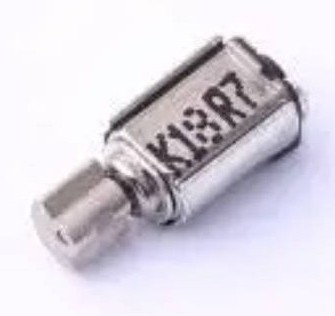
\includegraphics[width=0.35\textwidth]{images/unit7/vibration-motor.jpg}
  \caption{震动马达实物图}
  \label{fig:unit7_vibration_motor}
\end{figure}

在开发过程中，振动马达通常通过系统服务——命令行进行调用，应用只需向系统发出振动请求，即可启动硬件执行振动动作。调用方式包括设置固定时长的振动、按照预定义模式振动以及停止振动操作。固定时长振动常用于简短提醒，例如通知到达、按键触发等场景；模式振动可以设置振动和暂停的节奏组合，用于区分不同的提示或状态；停止振动则是释放硬件资源或中断当前振动，以应对突发事件或用户操作中断。
\subsection{振动马达数据采集示例}
通过本书编写的统一接口，开发者无需关注底层驱动差异，即可在不同设备上实现一致的振动控制效果。

\begin{lstlisting}
#include <stdio.h>
#include <stdint.h>
#include <string.h>
#include <stdlib.h>
#include <unistd.h>
#include <getopt.h>

#include "hdf_log.h"                // 标准日志接口头文件
#include "gpio_if.h"                // GPIO标准接口头文件
// GPIO引脚序号
static uint16_t m_gpio_id = 0;
// GPIO引脚是否设置为输入，GPIO_DIR_OUT为输出，GPIO_DIR_IN为输入
static uint16_t m_gpio_dir = GPIO_DIR_IN;
// GPIO引脚的高低电平，GPIO_VAL_LOW为低电平，GPIO_VAL_HIGH为高电平
static uint16_t m_gpio_value = GPIO_VAL_LOW;
\end{lstlisting}

本程序主要用于 GPIO 控制，可实现对振动马达的驱动和调试。程序首先引入标准 C 库和系统调用头文件，并包含了 hdf_log.h 和 gpio_if.h 等硬件接口头文件，为 GPIO 操作和日志输出提供支持。同时定义了软件版本号、打印信息宏以及 GPIO 基本状态变量，包括引脚编号、方向（输入/输出）和电平（高/低），为后续 GPIO 控制提供基础配置。
\begin{lstlisting}
void main_help(char *cmd)
{
    printf("%s: platform device gpio\n", cmd);
    printf("Version: %s\n", SOFTWARE_VERSION);
    printf("%s [options]...\n", cmd);
    printf("    -g, --gpio          gpio id\n");
    printf("    -v, --value         the value of gpio, 0 is low, 1 is high\n");
    printf("    -o, --out           gpio dir set to out\n");
    printf("    -i, --in            gpio dir set to in\n");
    printf("    -h, --help          help info\n");
    printf("\n");
}
\end{lstlisting}

程序提供了 main_help 函数，用于显示命令行参数的帮助信息。通过该函数，用户可以查看程序版本、支持的参数选项以及各选项的用途，例如设置 GPIO 编号、方向以及输出电平等。该功能在振动马达调试过程中非常重要，可以帮助用户快速定位和控制指定马达，避免误操作，提高调试效率和安全性。

\begin{lstlisting}
int main(int argc, char* argv[])
{
    int32_t ret;

    // 解析参数
    parse_opt(argc, argv);
    printf("gpio id: %d\n", m_gpio_id);
    printf("gpio dir: %s\n", ((m_gpio_dir == GPIO_DIR_OUT) ? ("out") : ("in")));
    printf("gpio value: %d\n", m_gpio_value);

    if (m_gpio_dir == GPIO_DIR_OUT) {
        // GPIO设置为输出
        ret = GpioSetDir(m_gpio_id, GPIO_DIR_OUT);
        if (ret != 0) {
            PRINT_ERROR("GpioSetDir failed and ret = %d\n", ret);
            return -1;
        }

        // GPIO输出电平
        ret = GpioWrite(m_gpio_id, m_gpio_value);
        if (ret != 0) {
            PRINT_ERROR("GpioWrite failed and ret = %d\n", ret);
            return -1;
        }
    } else {
        // GPIO设置为输入
        ret = GpioSetDir(m_gpio_id, GPIO_DIR_IN);
        if (ret != 0) {
            PRINT_ERROR("GpioSetDir failed and ret = %d\n", ret);
            return -1;
        }

        // 读取GPIO引脚的电平
        ret = GpioRead(m_gpio_id, &m_gpio_value);
        if (ret != 0) {
            PRINT_ERROR("GpioRead failed and ret = %d\n", ret);
            return -1;
        }

        printf("GPIO Read Successful and GPIO = %d, value = %d\n", m_gpio_id, m_gpio_value);
    }

    return 0;
}
\end{lstlisting}

通过 parse_opt 函数，程序能够解析命令行输入的参数，并将用户指定的 GPIO 编号、方向和输出电平存储到全局变量中。函数支持长短参数混合输入，例如
\begin{lstlisting}[numbers=none]
./gpio_control -g 5 -v 0 -o或./gpio_control --gpio 5 --value 0 --out
\end{lstlisting}

将 GPIO 输出设置为低电平，断开电源，停止振动马达。

\begin{lstlisting}[numbers=none]
./gpio_control -g 4 -i或./gpio_control --gpio 4 --in
\end{lstlisting}

-i 或 --in 设置 GPIO 为输入模式。程序会读取 GPIO 4 当前电平并输出，例如：
\begin{lstlisting}[numbers=none]
GPIO Read Successful and GPIO = 4, value = 0
\end{lstlisting}

命令行极大地方便了在不同测试环境下灵活控制振动马达。用户可以通过参数快速设置马达的震动状态，例如高电平启动马达，低电平停止马达，实现不同振动模式的测试。


在实际应用中，为了保证用户体验和系统稳定性，振动操作往往结合逻辑判断使用。例如，当应用检测到摇动动作或特定事件触发时，振动马达可以以短促、规律的振动反馈用户操作完成；在连续提醒场景中，可以通过模式振动传递复杂信息，如不同节奏表示不同等级的提示。此外，振动效果的实现还涉及硬件性能和功耗管理，需要合理选择振动时长和频率，以避免设备过热或电量快速消耗。

开发者在调试振动马达时，可以通过日志输出确认命令执行状态，也可结合界面交互观察振动效果。若设备未响应振动请求，需检查权限声明是否完整，例如应用是否获得系统振动权限，同时确保硬件接口未被其他应用占用。在一些复杂场景下，可通过模拟不同振动模式验证触觉反馈的可辨识性和舒适度，从而优化用户体验。

通过本任务的学习，读者能够掌握振动马达在 OpenHarmony 北向应用中的基本控制方法，包括启动、停止及模式设定，并理解振动操作在交互逻辑中的应用价值。掌握这些技能后，开发者可以在智能终端中实现多样化的触觉反馈，结合传感器数据进一步实现事件驱动的智能响应，为用户提供直观且丰富的交互体验。
\section{麦克风扬声器控制与调试}
\subsection{麦克风扬声器功能简介}
麦克风和扬声器是智能终端中最基础的音频输入输出设备，它们不仅承担语音交互、音频播放的功能，也是实现远程控制、智能语音助手以及多媒体交互的核心硬件。在开源鸿蒙（OpenHarmony）北向应用开发中，系统为开发者提供了统一的音频接口，使应用能够完成麦克风采集、音频播放以及音量和效果调节，从而构建完整的音频交互链路。

在麦克风数据采集方面，应用通过系统音频服务注册录音任务，系统随后将实时音频流推送给应用层。开发者可以设置采样率、声道数以及编码格式等参数，以满足不同场景的需求。例如，在语音识别或环境声音监测中，较高的采样率和双声道采集可以提供更清晰、更完整的音频信息，而在低功耗或带宽受限场景下，则可选择较低采样率以节省资源。麦克风采集的数据通常会进行简单的预处理，例如滤噪、归一化和增益调节，以保证音频输入的稳定性和清晰度。

扬声器控制方面，应用可以通过系统提供的播放接口加载音频文件或实时音频流，实现播放、暂停、停止以及音量调节等操作。在多媒体应用中，扬声器通常与界面或操作事件联动，例如消息提示音、操作反馈音或多媒体播放，如图\ref{fig:unit7_index}所示。

\begin{figure}[H]
  \centering
  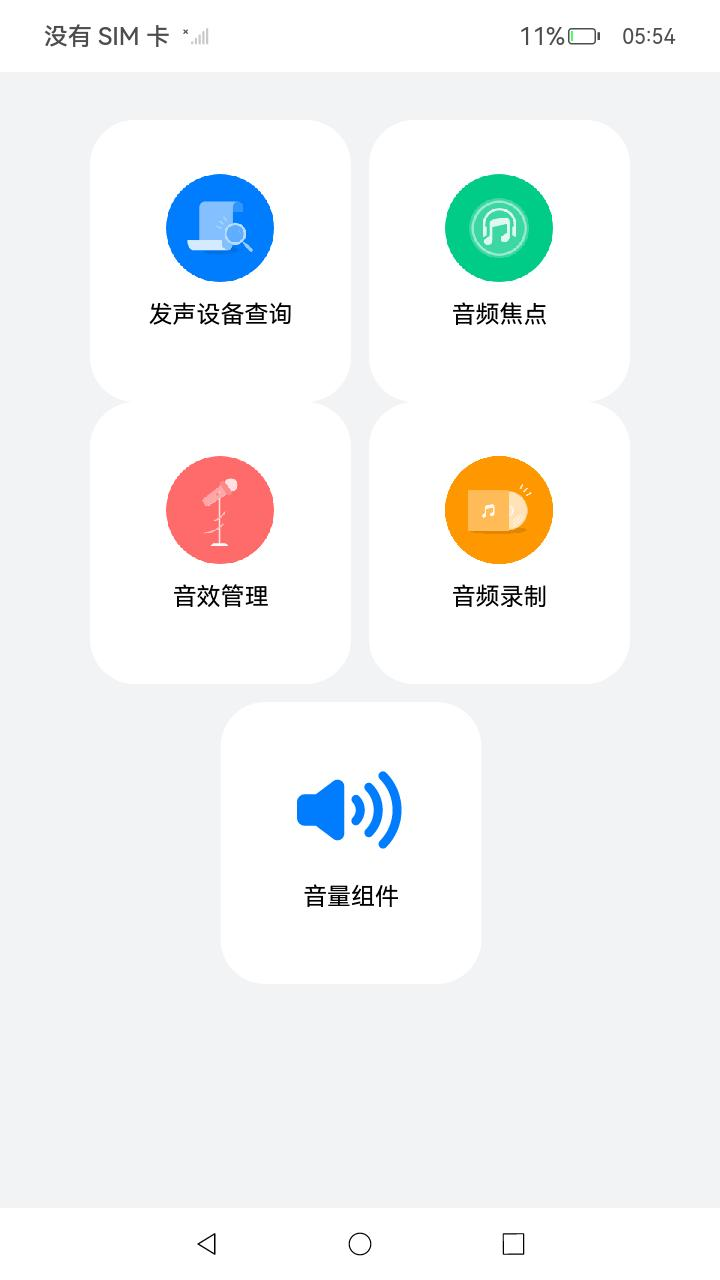
\includegraphics[width=0.24\textwidth]{images/unit7/index.png}
  \caption{主页}
  \label{fig:unit7_index}
\end{figure}

在控制策略上，应用可以结合逻辑事件调整播放模式和音量，使音频反馈与用户操作或系统状态保持一致。此外，开发者在调试阶段需要关注音频设备的占用状态以及权限声明，确保在调用麦克风或扬声器时不会被系统限制或其他应用占用。

为了增强应用的音频交互效果，麦克风与扬声器常结合其他传感器或触觉反馈组件使用。例如，语音控制场景中，用户通过麦克风输入指令，系统识别后通过扬声器进行语音反馈，同时可以结合振动马达提供触觉提示，从而实现多感官的交互体验。在实验和调试过程中，开发者可以通过日志和界面提示实时监控音频采集和播放状态，验证音频效果是否符合预期，并针对不同设备调整采样率、音量和缓冲策略，以优化性能和用户体验。
\subsection{麦克风扬声器数据采集与调试}
通过本任务的学习，读者能够掌握在 OpenHarmony 北向应用中完成音频采集和播放的基本方法，理解麦克风和扬声器的协同工作原理，并能够将音频输入输出与传感器数据或振动反馈结合，实现更丰富的智能交互应用。这为后续任务中的多通道设备控制和综合智能系统开发奠定了坚实的基础。
\section{RGB灯控制与调试}
\subsection{RGB灯功能简介}
RGB 灯是一种可通过单线数据总线控制的多色 LED 灯，其每颗灯珠包含红、绿、蓝三种发光二极管，通过调节亮度比例可以显示几乎所有颜色，如图\ref{fig:unit7_ws2812}所示。在智能设备、可穿戴设备、桌面装饰以及物联网终端中，RGB 灯常用于状态指示、报警反馈或视觉装饰效果。WS2812 系列是市场上常用的智能 RGB 灯，具有高度集成、驱动简便和单线串联控制的特点，北向应用开发者可以通过 OpenHarmony 提供的 GPIO 或 PWM 接口，结合专用驱动程序，实现对灯带的颜色显示、亮度调节和动态效果控制。

\begin{figure}[H]
  \centering
  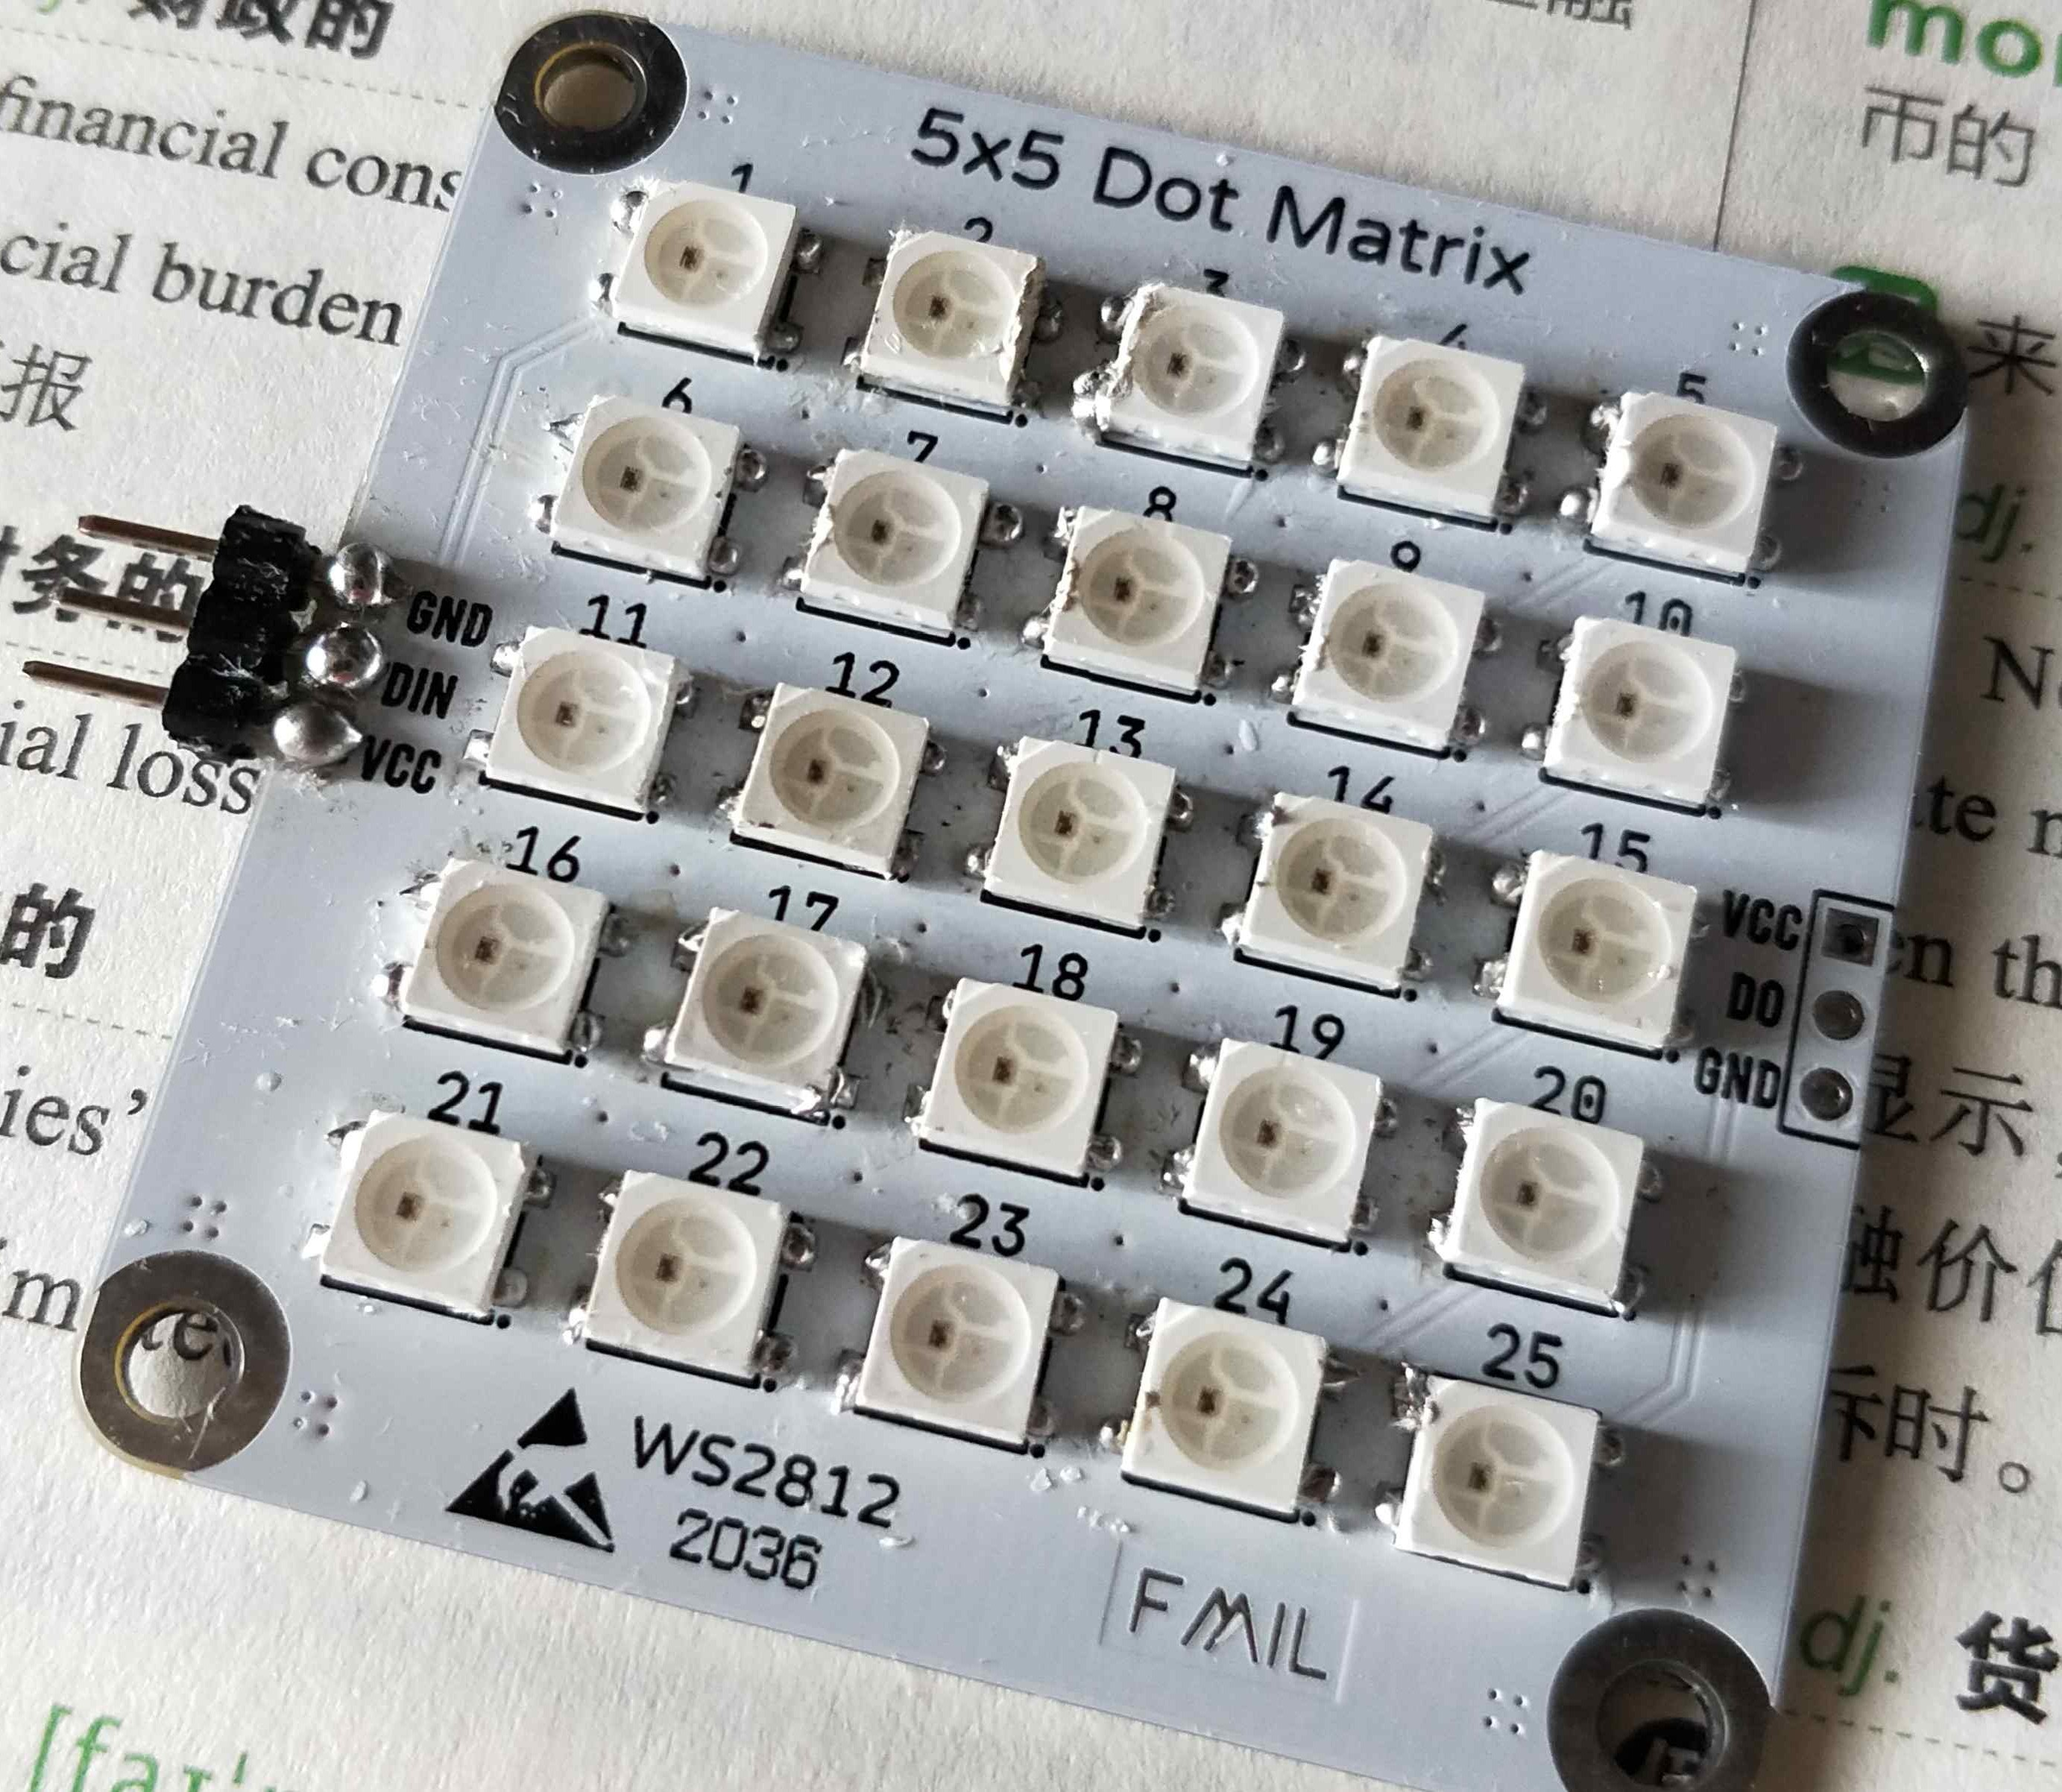
\includegraphics[width=0.8\textwidth]{images/unit7/ws2812.jpeg}
  \caption{RGB灯实物图}
  \label{fig:unit7_ws2812}
\end{figure}

在开发过程中，WS2812 灯的控制逻辑与应用状态紧密关联。每颗灯珠通过单线串联通信，可以设置独立颜色，形成丰富的灯光效果。开发者可以通过驱动接口发送数据帧，控制每个灯珠的红、绿、蓝亮度，从而实现颜色组合、闪烁、渐变和流水灯等效果。WS2812 灯的时序要求较高，通常需要精确控制数据输出的时间间隔，因此在北向应用中，通常会使用底层硬件定时器或专用控制库来保证数据传输稳定性。

实际应用中，RGB 灯不仅用于简单的视觉显示，更常结合传感器数据或系统事件，实现智能状态反馈。例如，当设备检测到温度超标、传感器异常或用户触发特定事件时，可以通过 RGB 灯的颜色变化和动态效果向用户提供直观提示。开发者可以设置红色表示错误或警告，绿色表示正常状态，蓝色或其他颜色用于提示特定模式或交互效果。通过调整亮度和颜色过渡，WS2812 灯能够实现流畅的视觉效果，增强设备的交互体验和美观度。

在调试过程中，开发者需要确认 GPIO 接口或 PWM 通道配置正确，并确保驱动库能够按照 WS2812 的时序要求发送数据。同时，需检查串联灯珠的数量与地址映射，避免颜色显示错位或灯珠不亮的问题。通过逐步测试单颗灯、局部灯组到整条灯带的效果，开发者可以验证动态效果是否符合预期，并优化颜色过渡、亮度调节和动画效果，使 RGB 灯的应用更加稳定和美观。
\subsection{WS2812 RGB 灯数据调试}
通过本任务的学习，读者能够掌握 WS2812 RGB 灯在 OpenHarmony 北向应用中的控制方法，包括单灯或灯带的颜色设置、亮度调节及动态效果实现，并理解其在智能终端中的应用价值。
\begin{lstlisting}
#include <stdio.h>
#include <stdint.h>
#include <string.h>
#include <stdlib.h>
#include <unistd.h>
#include <getopt.h>

#include "hdf_log.h"
#include "spi_if.h"                 // SPI标准接口头文件

// 定义版本号
#define SOFTWARE_VERSION            "V1.0"
// 定义字符串长度
#define STRING_MAXSIZE              128
\end{lstlisting}

该段主要包含了标准库和 SPI 驱动头文件的引用，同时定义了程序版本号、字符串长度常量以及调试信息打印宏。PRINT_INFO 和 PRINT_ERROR 宏可在程序执行过程中输出调试信息和错误信息，方便定位问题。
\begin{lstlisting}
#define RED_INDEX   0
#define GREEN_INDEX 1
#define BLUE_INDEX  2

#define WS2812_1    0xfc
#define WS2812_0    0xe0

static uint32_t m_spi_busNum = 3;       // SPI总线号
static uint32_t m_spi_csNum = 0;        // SPI片选号
static uint32_t m_spi_maxSpeedHz = 8000000;
static uint16_t m_spi_mode = 0;         // SPI模式
static uint8_t m_spi_transferMode = SPI_POLLING_TRANSFER;
static uint8_t m_spi_bitsPerWord = 8;   // 数据位宽

DevHandle g_spi_handle = NULL;

unsigned char COLOR[8][3]=
{
    {255, 0 , 0 },  //红色
    {255,255, 0 },  //黄色
    { 0 , 0 ,255},  //蓝色
    { 0 ,255, 0 },  //绿色
    { 0 ,255,255},  //青色
    {255, 0 ,255},  //紫色
    {255,255,255},  //白色
    { 0 , 0 , 0 }   //黑色
};

typedef enum
{
    RED = 0,
    YELLOW,
    BLUE,
    GREEN,
    CYAN,
    PURPLE,
    WHITE,
    BLACK
} COLOR_ENUM;

struct ws2812_color_arry {
    const char *color_str;
    COLOR_ENUM color_enum;
} g_ws2812_color_arry[] = {
    #define COLOR_DESC(col) {#col, col},
    COLOR_DESC(RED)
    COLOR_DESC(YELLOW)
    COLOR_DESC(BLUE)
    COLOR_DESC(GREEN)
    COLOR_DESC(CYAN)
    COLOR_DESC(PURPLE)
    COLOR_DESC(WHITE)
    COLOR_DESC(BLACK)
    #undef COLOR_DESC
    {NULL, 0}
};

static uint8_t g_color, g_led_num;
\end{lstlisting}

本段定义了 WS2812 LED 的 SPI 数据编码（WS2812_1 和 WS2812_0），SPI 总线和设备配置参数，以及 LED 颜色数组和枚举类型。同时定义了一个颜色映射表 g_ws2812_color_arry，用于将命令行输入的颜色字符串映射到枚举值，方便在程序中使用。
\begin{lstlisting}
static int ws2812_test_spi_write(unsigned char *rgb)
{
    unsigned char data[24];
    unsigned char i, bit;
    unsigned char index = 0;
    int ret;
    struct SpiMsg msg = {0};

    msg.wbuf = data;
    msg.len = 24;
    for (i = 0; i < 8; i++) // GREEN
    {
        bit = ((rgb[GREEN_INDEX] << i) & 0x80);
        data[index] = (bit == 0x80) ? 0xfc : 0xe0;
        index++;
    }
    for (i = 0; i < 8; i++) // RED
    {
        bit = ((rgb[RED_INDEX] << i) & 0x80);
        data[index] = (bit == 0x80) ? 0xfc : 0xe0;
        index++;
    }
    for (i = 0; i < 8; i++) // BLUE
    {
        bit = ((rgb[BLUE_INDEX] << i) & 0x80);
        data[index] = (bit == 0x80) ? 0xfc : 0xe0;
        index++;
    }

    ret = SpiTransfer(g_spi_handle, &msg, 1);
    if (ret != 0) {
        PRINT_ERROR("SpiTransfer failed and ret = %d\n", ret);
        return -1;
    }

    return 0;
}

static void ws2812_test_demo(uint8_t color, uint8_t led_num, uint8_t bright_level)
{
    unsigned char rgb[3];
    int i;

    rgb[0] = COLOR[color][0] & bright_level;
    rgb[1] = COLOR[color][1] & bright_level;
    rgb[2] = COLOR[color][2] & bright_level;

    for (i = 0; i < led_num; ++i) {
        ws2812_test_spi_write(rgb);
    }
}
\end{lstlisting}

该段包含两个核心函数：ws2812_test_spi_write()：将一个 LED 的 RGB 数据按 WS2812 协议编码为 SPI 数据并发送。ws2812_test_demo()：根据指定颜色和 LED 数量，循环调用 SPI 写函数，实现点亮多颗 LED。
\begin{lstlisting}
static void ws2812_test_print_help(void)
{
    int i;
    printf("Please use ws2812_test ");
    printf("<");
    for (i = 0; g_ws2812_color_arry[i].color_str != NULL; ++i) {
        if (i != 0) {
            printf("|");
        }
        printf("%s", g_ws2812_color_arry[i].color_str);
    }
    printf("> <led_num>\n");
}

static int ws2812_test_spi_init(void)
{
    int32_t ret = 0;
    struct SpiCfg cfg;
    struct SpiDevInfo dev;
    uint8_t data[24*10] = {0};

    dev.busNum = m_spi_busNum;
    dev.csNum = m_spi_csNum;
    g_spi_handle = SpiOpen(&dev);
    if (g_spi_handle == NULL) {
        PRINT_ERROR("SpiOpen failed\n");
        return -1;
    }

    ret = SpiGetCfg(g_spi_handle, &cfg);
    if (ret != 0) {
        PRINT_ERROR("SpiGetCfg failed and ret = %d\n", ret);
        SpiClose(g_spi_handle);
        return -1;
    }

    cfg.maxSpeedHz = m_spi_maxSpeedHz;
    cfg.mode = m_spi_mode;
    cfg.transferMode = m_spi_transferMode;
    cfg.bitsPerWord = m_spi_bitsPerWord;

    ret = SpiSetCfg(g_spi_handle, &cfg);
    if (ret != 0) {
        PRINT_ERROR("SpiSetCfg failed and ret = %d\n", ret);
        SpiClose(g_spi_handle);
        return -1;
    }

    SpiWrite(g_spi_handle, data, sizeof(data));
    return 0;
}

int main(int argc, char* argv[])
{
    int i;

    if (argc != 3) {
        ws2812_test_print_help();
        return -1;
    }
    for (i = 0; g_ws2812_color_arry[i].color_str != NULL; ++i) {
        if (strcmp(g_ws2812_color_arry[i].color_str, argv[1]) == 0) {
            g_color = g_ws2812_color_arry[i].color_enum;
            break;
        }
    }
    if (g_ws2812_color_arry[i].color_str == NULL) {
        ws2812_test_print_help();
        return -1;
    }
    g_led_num = (uint8_t)atoi(argv[2]);
    PRINT_INFO("color=[%s],led_num=[%d]\n", g_ws2812_color_arry[g_color].color_str, g_led_num);

    ws2812_test_spi_init();
    ws2812_test_demo(g_color, g_led_num, 255);

    return 0;
}
\end{lstlisting}

ws2812_test_print_help()：打印命令行使用帮助，告诉用户如何指定颜色和 LED 数量。ws2812_test_spi_init()：初始化 SPI 设备，配置总线号、片选号、最大频率、传输模式和数据位宽，并进行一次初始化写操作。main()：解析命令行参数，映射颜色字符串到枚举值，初始化 SPI 并点亮指定数量的 LED。

掌握这些技能后，开发者可以将 RGB 灯与传感器数据、振动反馈和音频输出结合，实现多感官的交互系统，为用户提供直观、丰富且动态的视觉体验。通过简单的命令行代码完成板载RGB灯的测试，
\begin{lstlisting}[numbers=none]
ws2812_test <color> <led_num>
\end{lstlisting}

\begin{lstlisting}[numbers=none]
./ws2812_test BLUE 5
\end{lstlisting}
通过此程序，读者能够完整了解命令行参数解析、SPI 外设初始化、WS2812 时序编码以及多灯珠控制的实现流程，为后续扩展动态灯效、亮度调节或多色组合奠定良好基础，最终板载RGB灯显示效果如图所示。该代码的功能LED 会显示蓝色，点亮 5 个。

当用户设置错误的颜色和LED数量时，例如。
\begin{lstlisting}[numbers=none]
./ws2812_test ORANGE 3
\end{lstlisting}

程序会提示用户输入有效的颜色和 LED 数量。
\begin{lstlisting}[numbers=none]
Please use ws2812_test <RED|YELLOW|BLUE|GREEN|CYAN|PURPLE|WHITE|BLACK> <led_num>
\end{lstlisting}